\subsection{Model fitting}
\label{subsec:fitting}
We employed a Markov Chain Monte Carlo (MCMC) script to fit the coefficients of a polynomial model for $r(M_c)$. The MCMC uses the smoothing prior as defined in section \ref{subsec:likelihood}. We performed a least square fit first in order to obtain the initial guess for the coefficients of the model.

The model we used is a polynomial of degree:
\begin{figure}[ht]
  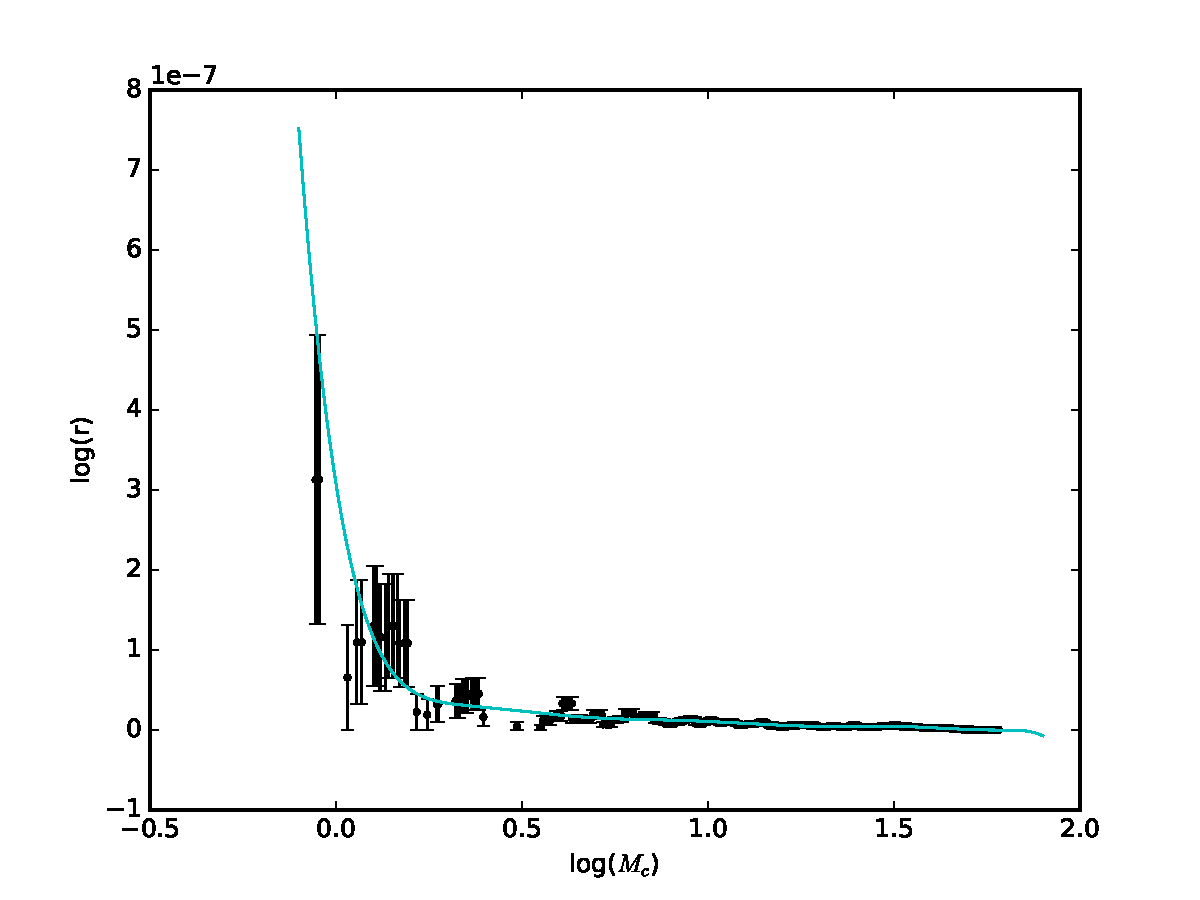
\includegraphics[width=\columnwidth]{img/line-MCMC.pdf}
  \caption{The cyan line is the best fit from MCMC.}
  \label{fig:line_MCMC}
\end{figure}